\section{Method}
\label{sec:method}

\subsection{Task: Evidence-Grounded Document-Level Relation Extraction}
\label{sec:task}

Given a document $D = \{s_1, \ldots, s_n\}$ consisting of $n$ sentences and a set of entities $\mathcal{E}$ identified within $D$, the task of evidence-grounded document-level relation extraction (DocRE) requires predicting, for each entity pair $(e_h, e_t) \in \mathcal{E} \times \mathcal{E}$, a relation $r \in \mathcal{R} \cup \{\texttt{NA}\}$ together with a set of supporting evidence sentences $E \subseteq D$. Standard DocRE predicts only the triple $(e_h, r, e_t)$; the evidence-grounded formulation also requires $E$, which grounds each prediction in specific textual support (Figure~\ref{fig:overview}).

\begin{figure}[t]
\centering
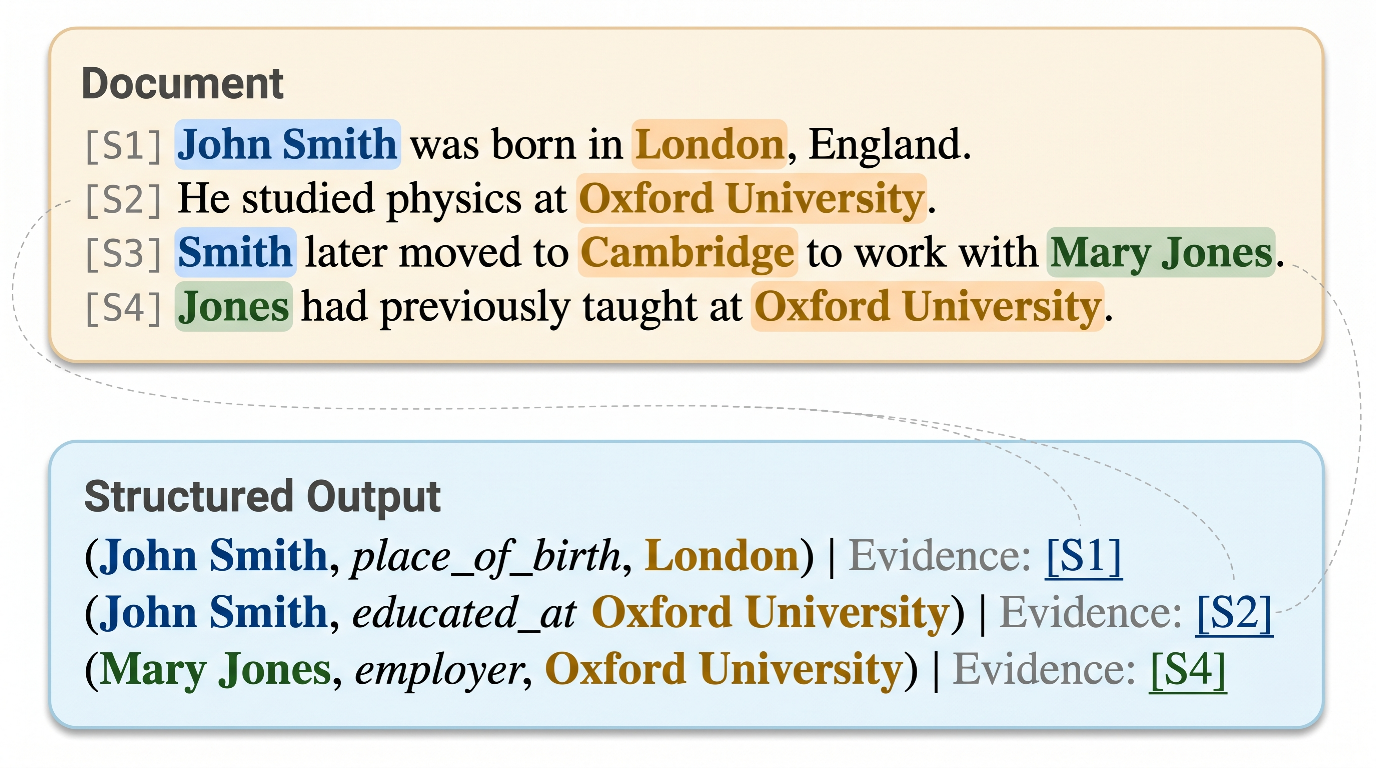
\includegraphics[width=\columnwidth]{fig_task_example.pdf}
\caption{Evidence-grounded DocRE example. Given a document with entity mentions, the model jointly predicts relation triples and supporting evidence sentences in a single structured output.}
\label{fig:task_example}
\end{figure}

In our LLM-based approach, the model generates structured outputs that jointly encode both components. For each predicted relation, the output follows the format \texttt{(head, relation, tail) | Evidence: [S$i$][S$j$]}, requiring the model to produce complete evidence references inline with each triple rather than as a separate retrieval step. This design contrasts with encoder-based evidence methods such as SAIS~\citep{xiao2022sais} and DREEAM~\citep{ma2023dreeam}, which frame evidence identification as sentence-level binary classification. Because classification over a fixed sentence set does not increase output length, these methods incur no generation overhead. Our LLM formulation requires additional tokens for each evidence reference, creating a generation burden that scales with the number of predicted triples and their evidence sentences. This scale-dependent cost is the central phenomenon we investigate.


\subsection{Supervised Fine-Tuning Baseline}
\label{sec:sft}

We fine-tune all models with Low-Rank Adaptation (LoRA) \citep{hu2022lora} at rank $r{=}64$ and scaling factor $\alpha{=}128$, applied to all linear projections (attention and feed-forward). The training data consists of DocRED~\citep{yao2019docred} training documents converted to the structured output format described above, where each example maps a document and its entity set to the complete set of relation triples with evidence annotations. We also train a \emph{no-evidence} variant under identical configuration but with evidence references removed from the output format, producing only \texttt{(head, relation, tail)}. This variant serves as an upper bound on extraction performance by eliminating the generation cost of evidence, and allows direct measurement of the evidence tax at each model scale. Detailed hyperparameters are reported in Appendix~\ref{sec:hyperparams}.


\subsection{Optimization Paradigms}
\label{sec:paradigms}

We evaluate three post-SFT optimization paradigms that differ in how they incorporate quality signals from the CED scoring function (\S\ref{sec:ced}). Table~\ref{tab:paradigm_comparison} summarizes their key differences.

\begin{table}[t]
\centering
\caption{Comparison of post-SFT optimization paradigms. All three use CED scoring but differ in how quality signals reach the model.}
\label{tab:paradigm_comparison}
\small
\begin{tabular}{lccc}
\toprule
& \textbf{GRPO} & \textbf{DPO} & \textbf{RSFT} \\
\midrule
Signal type & Online RL & Implicit RL & Selection \\
CED role & Reward & Preference & Filter \\
Update & Gradient & Gradient & Supervised \\
Decoupling & Yes & Partial & None \\
\bottomrule
\end{tabular}
\end{table}

\paragraph{GRPO.}
Group Relative Policy Optimization~\citep{shao2024deepseekmath} is an online RL method that eliminates the need for a separate value network by computing advantages within groups of sampled outputs. For each training document, the policy generates $G$ candidate responses, which are scored by CED. The advantage of each response is computed relative to the group mean, and the policy is updated to increase the probability of above-average outputs. We test two configurations: QLoRA \citep{dettmers2023qlora} under 4-bit quantization, and bf16 full-precision LoRA, both with $G{=}8$ groups. Because GRPO applies gradient updates that directly optimize the reward signal, evidence quality and extraction accuracy compete for gradient capacity. We analyze this multi-objective tension in Section~\ref{sec:spectrum}.

\paragraph{DPO.}
Direct Preference Optimization~\citep{rafailov2023direct} reformulates RLHF~\citep{ouyang2022instructgpt} as a classification problem over preference pairs, without explicit reward models. We construct preference data from the SFT model's sampled outputs: for each document, the response with the highest CED score is labeled as preferred and the lowest-scoring response as rejected. DPO then adjusts the policy to increase the log-probability ratio between preferred and rejected completions. We train for 1 and 3 epochs to observe the temporal dynamics of evidence-extraction trade-offs under implicit optimization.

\paragraph{RSFT.}
Rejection Sampling Fine-Tuning is a single-round variant of iterative self-improvement methods such as STaR~\citep{zelikman2022star}. The procedure is straightforward: for each SFT checkpoint, the corresponding model generates $N{=}8$ candidate outputs per training document, each candidate is scored by CED, and only the top-$k{=}1$ response is retained as training data. In our primary experiments (4B, 8B, LLaMA-8B), all RSFT seeds share the same SFT s42 checkpoint and the same CED-scored training data; only the LoRA initialization and data shuffling seeds differ during the final fine-tuning stage. At 14B, seed-matched SFT checkpoints are used. We use $k{=}1$ (best-of-$N$) selection throughout all experiments, selecting the single highest-scoring candidate per document. This yields approximately 3,000 training examples per model (one per document; exact counts vary slightly by model due to generation failures). Unlike GRPO and DPO, RSFT does not apply gradient-based optimization pressure toward a reward signal. Instead, it improves training data quality through filtering: the model trains on its own best outputs rather than all outputs. This distinction is critical because discrete selection over complete outputs cannot exploit the extraction-evidence trade-off that gradient methods find. The contribution of RSFT in our setting is not the framework itself, which is well-established, but its application to evidence-grounded DocRE with CED as a domain-specific quality filter.


\subsection{Contrastive Evidence Discrimination}
\label{sec:ced}

\begin{figure}[t]
\centering
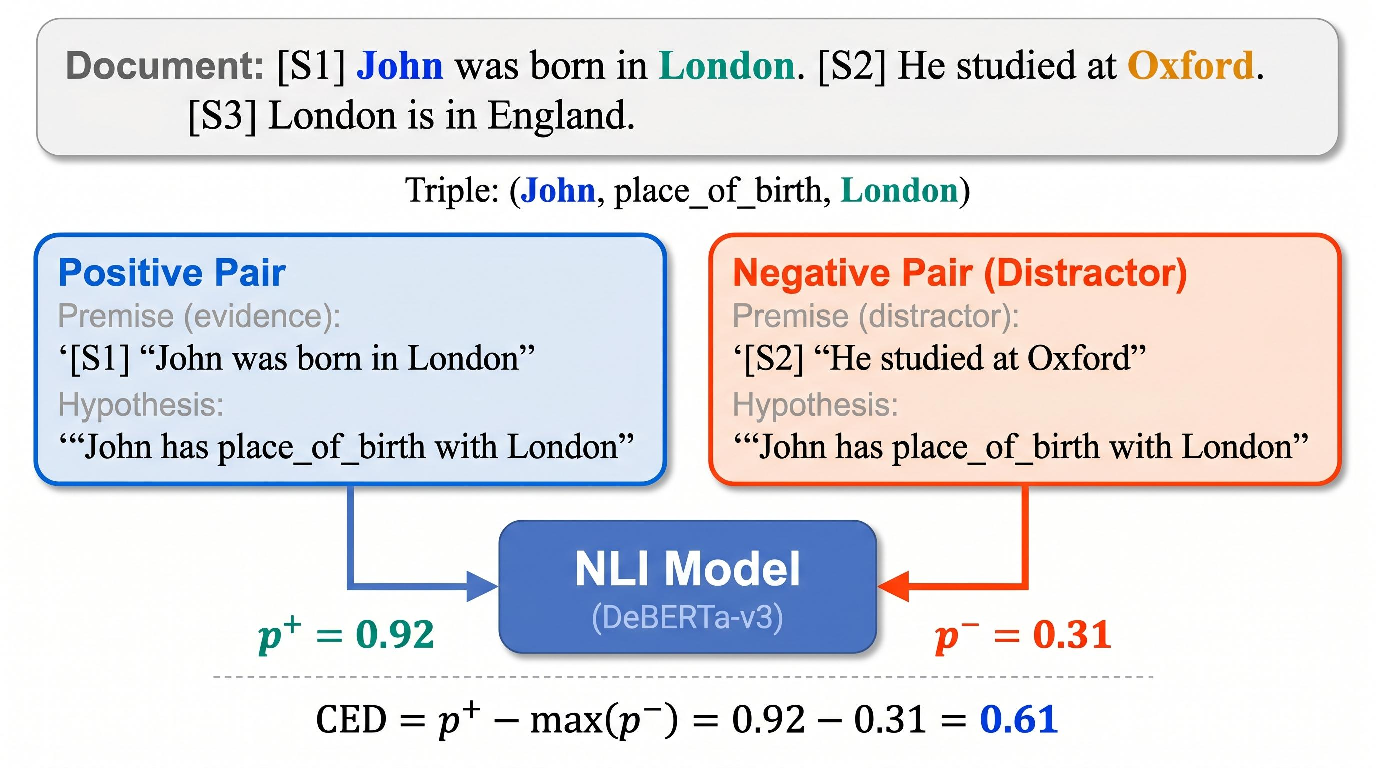
\includegraphics[width=\columnwidth]{fig_ced_scoring.pdf}
\caption{CED scoring example. The positive pair (evidence $\to$ hypothesis) yields high entailment; the contrastive distractor (entity-sharing non-evidence) yields low entailment. CED measures the margin between them.}
\label{fig:ced_scoring}
\end{figure}

CED is a scoring function that evaluates the faithfulness of predicted evidence sentences to their associated relation triples. It builds on Natural Language Inference (NLI) to measure whether evidence actually entails the predicted relation, rather than merely co-occurring with the relevant entities.

For a predicted triple $(e_h, r, e_t)$ with evidence sentences $E$, CED constructs a positive NLI pair: the premise is the concatenation of sentences in $E$, and the hypothesis is a natural-language verbalization of the relation (e.g., ``$e_h$ has relation $r$ with $e_t$''). An NLI model based on DeBERTaV3 \citep{he2023debertav3} (\texttt{cross-encoder/nli-deberta-v3-base}) produces an entailment probability $p^+$ for this pair. The contrastive component introduces hard negatives drawn from the same document. For each triple, we collect sentences that mention $e_h$ or $e_t$ but are not in the predicted evidence set. These entity-sharing distractors serve as negative premises, and the NLI model scores each to obtain $p^-_1, \ldots, p^-_m$. The CED score for a single triple is:
\begin{equation}
\text{CED}(e_h, r, e_t, E) = p^+ - \max_j \, p^-_j
\label{eq:ced}
\end{equation}
This formulation forces the scoring function to distinguish sentences that genuinely support the relation from sentences that merely mention the same entities. A high CED score indicates that the evidence provides relation-specific support beyond entity co-occurrence.

The document-level CED score aggregates over all predicted triples, weighted by extraction correctness: triples that match ground-truth relations contribute their CED scores, while incorrect triples receive zero credit. This coupling ensures that CED rewards both faithful evidence and accurate extraction jointly.

We also evaluate a \emph{flat-NLI} baseline that uses only the positive entailment score $p^+$ without the contrastive term. CED and flat-NLI produce comparable RSFT outcomes (mean Rel-F1 difference of 0.02pp across available seeds; Section~\ref{sec:analysis}), confirming that the contrastive formulation is not essential for data selection quality. We adopt CED as the default because its per-triple discrimination scores support interpretable error analysis.


\subsection{Evidence-Decoupling Ratio}
\label{sec:edcr}

For analysis, we define the Evidence-Decoupling Ratio (EDCR) as a diagnostic metric that quantifies the degree of misalignment between a model's extraction and evidence capabilities. EDCR is not a training component; it serves purely as an analytical tool for comparing optimization methods.

EDCR is defined as the distractor citation rate across all predicted triples:
\begin{equation}
\text{EDCR} = \frac{\sum_{i} |E_i^{\text{pred}} \setminus E_i^{\text{gold}}|}{\sum_{i} |E_i^{\text{pred}}|}
\label{eq:edcr}
\end{equation}
where the sum ranges over all predicted triples with at least one evidence citation. $E_i^{\text{pred}}$ is the set of evidence sentences cited for predicted triple $i$, and $E_i^{\text{gold}}$ is the corresponding gold evidence (empty for false-positive predictions). EDCR thus measures the fraction of all cited evidence that does not appear in the gold evidence for the associated triple.

A model with many false-positive triples will have high EDCR because all evidence for incorrect triples counts as distractor; even among correct triples, citing irrelevant sentences inflates the numerator. Conversely, accurate extraction with faithful evidence yields low EDCR. This dual sensitivity makes EDCR a natural diagnostic for extraction-evidence decoupling.

EDCR operates at two diagnostic levels. At the method level, comparing EDCR across seven unique method configurations reveals a negative correlation with Rel-F1 (Spearman $\rho{=}{-}0.96$, $n{=}7$, $p{<}0.001$). Because EDCR is mechanically influenced by false-positive triples (which share determinants with Rel-F1), this correlation should be interpreted as a diagnostic pattern rather than an independent discovery; its primary value lies in per-relation analysis. We validate EDCR's diagnostic utility through per-relation analysis (\S\ref{sec:analysis}), which avoids the shared-component concern present in cross-method correlation. At the per-relation level, computing EDCR for individual relation types reveals a robust negative correlation with Rel-F1 ($\rho{=}{-}0.79$, $n{=}76$, $p{<}0.001$) that is independent of Evi-F1 ($\rho{=}{-}0.06$, $p{=}0.58$). This independence means EDCR captures relation-specific extraction-evidence misalignment that aggregate evidence metrics miss. The SFT baseline EDCR (0.6797, three-seed mean) reflects the inherent distractor rate under standard training; EDCR values substantially exceeding this level (e.g., GRPO QLoRA at 0.9876) indicate RL-induced decoupling beyond what evidence production alone explains, while values below the baseline (e.g., RSFT at 0.6487) reflect improved co-optimization.
